\chapter{Analogy-preserving functions}

\cite{HugPraRicSerECAI16} have proved that this kind of analogical
classification process can be formalized via two conceptual steps: first an
{\it analogical  extension} of the training set is performed (as detailed in
Section \ref{analogy}), and then a $k$-NN-like algorithm is applied to this
extended training set.  As expected, the accuracy of the analogical classifier
greatly depends on the quality of the extension. In this  paper, we introduce
the class of Analogy Preserving (AP) functions which ensure an error-free
extension.

Our paper is structured as follows. In Section \ref{extending} we overview
different methods currently used for extending a sample set.  In Section
\ref{analogy} we recall the basics of analogy and its counterpart in Boolean
logic (namely the analogical proportions), pointing out the existence of two
potential modelings. We also recall the process of
extending a sample set via analogy and introduce the notion of AP functions.
Section \ref{class_of_ap_functions} is devoted to a theoretical
characterization of AP functions. In section \ref{approximate_ap_functions} we
define and empirically investigate \textit{approximate} AP functions. We then
show their suitability for training set extension.

\section{Extending a training set}\label{extending}
Extension of a sample set (or training set) of a given universe $\mathcal{X}$
is a simple idea to improve generalization power. The more examples you have,
the better you learn! The point is then to add to the sample set $S$ some new
examples, but we have to do that in a way that preserves the \textit{quality}
of $S$.

Formally, we start with a set $S= \{x^{(i)} \in \mathcal{X}| i \in [1,n]\}$ of
examples ($n$ is supposed to be small), where $x^{(i)}$ is an
element of a Cartesian product $\mathcal{X} = X_1 \times \ldots \times X_m$.
For each element  $x^{(i)} \in S$, we associate a target  $f(x^{(i)})=y^{(i)}
\in Y$.  In the case of regression, $y^{(i)} \in \mathbb{R}$, and in the case
of classification $y^{(i)}$ belongs to a finite set and is called a class
or a \textbf{label}.

Several methods have been proposed for extending a sample set with new
examples. We may build a new example starting from
1, 2 or 3 known examples.
\begin{enumerate}
\item With one example, a natural way to proceed is to use the classical
  neighborhood approach: given one  example $(a,f(a))$, we can generate a new
    example $(b,f(b))$ where  $b$ is not too far from $a$ and $f(b)$ is not too
    far from $f(a)$. In the classification case, $f(b)$ may be chosen as
    $f(a)$.
\item With two examples, the previous option is still available and leads to
  interpolate the new example from the two given ones.  A somehow different
    option is the Feature Knockout procedure \cite{WolMar04}, which amounts
    to build a third example obtained by modifying a randomly chosen feature
    of the first example with that of the second one.  This way to
    proceed enjoys nice properties and appears to be equivalent to a popular
    regularization (Tikhonov) technique in the case of linear regression.  A
    related idea is used in a recent proposal \cite{BouPraRicECAI16} which
    introduces a measure of oddness w.r.t. a class that is computed on the
    basis of pairs made of two nearest neighbors in the same class; this is
    equivalent to replace the two neighbors by a fictitious representative of
    the class.

\item With three examples $(a,f(a)), (b,f(b)), (c,f(c))$, the previous options
  remain available and lead to build a fourth example which is somehow
    in-between the three other ones: we still have some kind of interpolation.
    A quite different idea is to extrapolate the fourth item on the basis of
    analogical proportion \cite{BayMouMicAnqECML07}.  In this perspective,
    this fourth element is not necessarily in the neighborhood of the three
    others.
\end{enumerate}
In this paper, we investigate this last option in depth.

\subsection{Analogy-preserving functions}\label{analogy-preserv}

\begin{definition}
  We say that $\mathbf{E}_S(f)$ is {\bf sound} if
  $\albl{\mathbf{x}}_f=f(\mathbf{x})$, for every $\mathbf{x} \in
  \mathbf{E}^*_S(f)$. Also, if $\mathbf{E}_S(f)$ is sound for all $S \subseteq
  \mathbb{B}^m$, we say that $f$ is {\bf Analogy Preserving} (AP).
\end{definition}

\noindent
Proposition \ref{equivalent_def} gives an equivalent definition of AP
functions.

\begin{proposition}\label{equivalent_def}
  A function $f \colon \mathbb{B}^m \to \mathbb{B}$ is AP iff for every
  $\mathbf{a}, \mathbf{b}, \mathbf{c}, \mathbf{d} \in \mathbb{B}^m$, $f$ suits
  the following requirement:
  $$
  \begin{cases}
    \mathbf{a} :  \mathbf{b} ::  \mathbf{c} :  \mathbf{d} \emph{ and }\\
  f(\mathbf{a}) :  f(\mathbf{b}) ::  f(\mathbf{c}) :  y \emph{ is solvable  }
  \end{cases}
  \implies y = f(\mathbf{d})
  $$
\end{proposition}
\begin{proof}
  If $f$ fulfills  this requirement, then it is clear from Section
  \ref{analogy-extension} that for any $S \subseteq
  \mathbb{B}^m$ and $\mathbf{x} \in \mathbf{E}^*_S(f)$, all the candidates $y$
  for $\albl{\mathbf{x}}_f$ are equal to $f(\mathbf{x})$, so
  $\albl{\mathbf{x}}_f$ will be invariably set to $f(\mathbf{x})$, which makes
  $f$ AP.

If $f$ does not suit this requirement, then there exist $\mathbf{a},
  \mathbf{b}, \mathbf{c}$, and $\mathbf{d} \in \mathbb{B}^m$ such that
  $\mathbf{a} : \mathbf{b} :: \mathbf{c} : \mathbf{d}$ but the solution $y$ to
  $f(\mathbf{a}) : f(\mathbf{b}) :: f(\mathbf{c}) : y$ is not equal to
  $f(\mathbf{d})$. Taking $S_0 = \{\mathbf{a}, \mathbf{b}, \mathbf{c}\}$ we
  obtain $\mathbf{E}^*_{S_0}(f) = \{\mathbf{d}\}$, and since $\albl{\mathbf{d}}_f = y
  \neq f(d)$, $\mathbf{E}_{S_0}(f)$ is not sound so $f$ is not AP.
\end{proof}

If $f$ is AP, then $\mathbf{E}_S(f)$ is sound for any $S$ so it is a relevant
extension of $S$ and can be used with full confidence for classification
purposes. In the rest of the paper, we will give a definite answer to the
following problem:

\begin{problem}\label{prob}
  Give a complete description of the functions $f\colon \mathbb{B}^m\to
  \mathbb{B}$ that ensure a sound extension $\mathbf{E}_S(f)$ for any sample
  set $S\subseteq \mathbb{B}^m$. In other words, identify all the AP
  functions.
\end{problem}

First note that many natural functions are not AP. Consider for example the
binary function $f(x_1,x_2)= x_1 \wedge x_2$, along with $\mathbf{a},
\mathbf{b}, \mathbf{c}, \mathbf{d} \in \mathbb{B}^2$ in Table
\ref{exampleNotAP}.  We have $\mathbf{a} : \mathbf{b} :: \mathbf{c} :
\mathbf{d}$ and $f(\mathbf{a}) : f(\mathbf{b}) :: f(\mathbf{c}) : y$ is
solvable, yet the solution is $y=0$, which  is different from $f(\mathbf{d})=1$
so $f$ is not AP. This actually comes from the fact that analogical proportions
are not stable by conjunction combination. It is also the case for the
disjunction \cite{PraRic14}.

\begin{table}[ht]
$\begin{array}{|c|cc|c|}
  \toprule
  ~ & x_1 & x_2 & f(\cdot) \\
  \midrule
  \mathbf{a} & 0 & 0 & 0\\
  \mathbf{b} & 0 & 1 & 0\\
  \mathbf{c} & 1 & 0 & 0\\
  \mathbf{d} & 1 & 1 & 1\\
  \bottomrule
\end{array}
$\bigskip
\caption{$f(x_1,x_2)= x_1 \wedge x_2$ is not AP.}
\label{exampleNotAP}
\end{table}

In the next section, we provide a complete description of AP functions and give
an answer to Problem \ref{prob}.

\section{The class of AP functions}
\label{class_of_ap_functions}

We first need to recall some basic notions in the theory of essential variables
of functions.

\subsection{Essential variables and sections of functions}

For $k\in [1,m]$, $\boldsymbol{\alpha}\in \mathbb{B}^m$, and $c \in
\mathbb{B}$, let ${\boldsymbol{\alpha}}_{k}^c$ be the tuple in $\mathbb{B}^{m}$
whose $i$-th component is set to $c$ if $i=k$, and to $\alpha_i$ otherwise.  A
variable $x_i$ is said to be \textbf{inessential} in $f\colon \mathbb{B}^m\to
\mathbb{B}$ if for all $\boldsymbol{\alpha} \in \mathbb{B}^m$ and $c \in
\mathbb{B}$, $f(\boldsymbol{\alpha}^c_i) = f(\boldsymbol{\alpha}^{\neg c}_i)$.
Otherwise, $x_i$ is said to be \textbf{essential} in $f$, or that $f$ depends
on $x_i$. In simple terms, an
essential variable is a variable that has the \textit{ability} to change the
value of $f$. For example in $f(x_1, x_2, x_3) = x_1 \wedge x_3$, $x_1$ and
$x_3$ are essential variables while $x_2$ is inessential.  We denote by
$\ess(f)$ the number of essential variables of $f$ (or \textbf{essential
arity}).

Two functions $f\colon \mathbb{B}^m\to \mathbb{B}$ and $g\colon \mathbb{B}^n\to
\mathbb{B}$ are said to be {\bf equivalent} if there exist two mappings
$\sigma\colon
[1,n]\to [1,m]$ and $\sigma'\colon [1,m]\to [1,n]$ such that
\begin{align*}
  f(x_1,\ldots , x_m)&=g(x_{\sigma(1)},\ldots,x_{\sigma(n)}) \text{ and} \\
   g(x_1,\ldots , x_n)&=f(x_{\sigma'(1)},\ldots,x_{\sigma'(m)}).
\end{align*}
In other words, $f$ and $g$ are equivalent if one can be obtained from the
other by permutation of variables, addition of inessential variables, or
identification of inessential variables. For example, $f(x_1, x_2, x_3) = x_1
\wedge x_3$ and $g(x_1, x_2)  = x_1 \wedge x_2$ are equivalent functions. Note
that two equivalent functions necessarily have the same number of essential
variables. For further background in the theory of essential variables of
functions, see \cite{CouceiroTCS08, CouceiroDM09, SalomaaAASF63, WillardDM96}.

In our demonstrations, we will use the following property:

\begin{property}\label{equivalent_functions}
Let $f\colon \mathbb{B}^m\to \mathbb{B}$ and $g\colon \mathbb{B}^n\to
  \mathbb{B}$ be equivalent functions. Then $f$ is AP if and only if $g$ is AP.
\end{property}

This can be verified by noting that as the analogy in $\mathbb{B}^m$ is defined
component-wise, the permutation of variables has no effect on the equation and
its solution. Also, manipulation of inessential variables do not change the
value of the function $f$, and thus the AP property still holds.

We now define the concept of \textbf{section} of a function, also known as a
\textit{restriction}, or equivalently as the result of \textit{partial
application} in computer science. Let $f$ be a function $\mathbb{B}^m\to \mathbb{B}$, and $(I,
J)$ be a partition of $[1, m]$. With $\mathbf{x}
\in \mathbb{B}^m$ and $\boldsymbol{\alpha} \in \mathbb{B}^{|I|}$, the $I$-section (or simply
section) $f^{\boldsymbol{\alpha}}_I \colon \mathbb{B}^{|J|} \to \mathbb{B}$ is the function that
is obtained after setting all variables in $I$ to the components of
$\boldsymbol{\alpha}$. Note that the arity of $f^{\boldsymbol{\alpha}}_I$ is
$|J|$, and that $\ess(f^{\boldsymbol{\alpha}}_I) \leq \ess(f)$.
For example, consider a function $f$ of three variables: $f(x_1,x_2, x_3) = (x_1
\wedge x_2) \lor x_3$. The section $f^{(1, 0)}_{\{1, 3\}}$ is defined as $f^{(1,
0)}_{\{1, 3\}}(x_2) = (1 \wedge x_2) \lor 0$.

A main result about sections that will be used in other proofs is stated in
Property \ref{section_preserve_wap}, which can be verified by noting that
$x:x::x:x$ for any $x \in \mathbb{B}$:

\begin{property}\label{section_preserve_wap}
If $f\colon \mathbb{B}^m\to \mathbb{B}$ is AP, then every section of $f$ is
also AP.  \end{property}

In the following, the AND operator `$\wedge$' will be denoted `$\cdot$' to fit
with an algebraic notation. Also, `$+$' will now denote the modulo-2 addition,
equivalent to the XOR operator. Note that $x + 1 = \neg x$.

\subsection{The affine functions}

We are now in a position to see some examples of AP functions. We will show that
any affine function is AP.

\begin{proposition}\label{affine_functions_are_wap}
Let $L$ be the class of all affine functions, i.e. functions of the form:
  $$f(x_1,\ldots , x_m)=\alpha_1\cdot x_1+\ldots +\alpha_m\cdot  x_m+\alpha,$$
  with $\alpha_1,\ldots, \alpha_m,\alpha\in \mathbb{B}$. Every affine function
  (also called linear when $\alpha = 0$) is AP.
\end{proposition}

\begin{proof}
Let $f \colon \mathbb{B}^m \to \mathbb{B} \in L$. Using the obvious fact that
  $f$ is AP  iff $f + 1 = \neg f$ is AP, we may assume without loss of generality that
  $\alpha = 0$. Also, considering that $f$ essentially depends on $n \leq m$
  variables ($n$ is then the number of $\alpha_i$ equal to $1$), $f$ is
  equivalent to the function $g \colon \mathbb{B}^n \to \mathbb{B}$ defined by
  $g(x_1, \cdots, x_n) = x_1 +  \cdots + x_n$. Using Property
  \ref{equivalent_functions}, we just need to prove that $g$ is AP to show that
  $f$ is also AP.

  This function $g$ has the remarkable property\footnote{This is the reason why affine
  functions lead to classification problems that are, in fact, highly
  \textbf{non} linearly separable.} that changing the value of any
  $x_i$ changes the value of $g$: $\forall _i, \quad g(x_1, \cdots, x_i, \cdots, x_n) =
  \neg g(x_1, \cdots, \neg x_i, \cdots, x_n)$. From this property, it is easy to
  see that:
  $$\forall \mathbf{x}, \mathbf{x}' \in \mathbb{B}^n, g(\mathbf{x}) =
  g(\mathbf{x}') \iff h(\mathbf{x}, \mathbf{x}') \text{ is even },$$
  where $h$ is still the Hamming distance function.

  Let $\mathbf{a}, \mathbf{b}, \mathbf{c}, \mathbf{d} \in \mathbb{B}^m$  such
  that the two hypothesis in the definition of AP are satisfied, i.e.
  $$
  \mathbf{a} : \mathbf{b} :: \mathbf{c} : \mathbf{d}\quad \text{and}\quad
  g(\mathbf{a}) : g(\mathbf{b}) :: g(\mathbf{c}) : y\quad  \text{is  solvable}.
  $$

  As the equation is solvable, Table \ref{truthTableAnalogy} tells us that
  there are three possibles cases (we will use Property
  \ref{hamming_analogy}):
  \begin{enumerate}
    \item $g(\mathbf{a}) = g(\mathbf{b})$, and in this case the solution is
      $y = g(\mathbf{c})$. As $g(\mathbf{a}) = g(\mathbf{b})$, then
      $h(\mathbf{a}, \mathbf{b})$ is even, and so is $h(\mathbf{c},
      \mathbf{d})$. Then, $g(\mathbf{c}) = g(\mathbf{d})$ so $y = g(\mathbf{d})$.
    \item $g(\mathbf{a}) = g(\mathbf{c})$, and in this case the solution is $y =
      g(\mathbf{b})$. As $g(\mathbf{a}) = g(\mathbf{c})$, then
      $h(\mathbf{a}, \mathbf{c})$ is even, and so is $h(\mathbf{b},
      \mathbf{d})$. Then $g(\mathbf{b}) = g(\mathbf{d})$ so $y =
      g(\mathbf{d})$.
    \item $\neg g(\mathbf{a}) = g(\mathbf{b}) = g(\mathbf{c})$, and in this
      case the solution is $y = g(\mathbf{a})$. As $g(\mathbf{b}) =
      g(\mathbf{c})$, then $h(\mathbf{b}, \mathbf{c})$ is even, and so is
      $h(\mathbf{a}, \mathbf{d})$. Then $g(\mathbf{a}) = g(\mathbf{d})$ so $y =
      g(\mathbf{d})$.
  \end{enumerate}

  The third case is only relevant for the Klein modeling. In all cases we have
  $y = g(\mathbf{d})$, thus showing that $g$ is AP, and so is any $f \in L$.
\end{proof}


\subsection{A complete description of AP functions}

We have seen that every affine function is AP. We will here give a stronger
result: the affine functions are the \textbf{only} AP functions.

For that we shall make use of the  polynomial representation of Boolean functions.
A \textbf{ monomial} is a term of the form:
$$
\mathbf{x}_I=\underset{i\in I}{\prod}x_i, $$ for some possibly empty finite set of
positive integers $I$, where $|I|$ is called the \textbf{degree} of
$\mathbf{x}_I$.   We take the convention that $1$ is the empty monomial
$\mathbf{x}_\emptyset $. A \textbf{ polynomial} is a sum of monomials and its
degree is the largest degree of its monomials.  It is well-known
\cite{StoneAlgebra36,ZhegalkinAlgebra27} that any function
$f:\mathbb{B}^m\rightarrow \mathbb{B}$ is uniquely represented by a polynomial,
also called the Algebraic Normal Form: $$f(x_1,\ldots,x_m)=\sum_{I\subseteq
\{1,\ldots,m\}}a_I\cdot \mathbf{x}_I$$ where each $a_I$ belongs to
$\mathbb{B}$. Note that the constant function $0$ is represented by
$a_\emptyset\cdot \mathbf{x}_\emptyset$ with $a_\emptyset =0$. The degree of a
function $f:\mathbb{B}^m\rightarrow \mathbb{B}$, denoted $d(f)$, is defined as
the degree of the unique polynomial representing $f$.

Note that the class of functions with degree at most $1$ is exactly the class
$L$ of affine functions, which are AP. We will show that the class of AP
functions is the class of affine functions by proving that if a function $f$ is
AP, then $d(f)\leq 1$. We first consider the case where $d(f) = 2$.

\begin{property} \label{degree_2_not_AP}
 Let $f\colon \mathbb{B}^m\to \mathbb{B}$ with $d(f)=2$. $f$ is not AP.
\end{property}
\begin{proof}
  Let's consider $f$ with $d(f) = 2$ and $\ess(f) >= 2$. We denote $\mathbf{x}_I$ one of the
  monomial of $f$ of degree $2$. We consider the section $f^{\mathbf{0}}_J$,
  where $J = [1, m] \setminus I$,  and $\mathbf{0}$ denotes the constant 0
  vector in $B^{|J|}$. All variables that are not part of the monomial
  $\mathbf{x}_I$ have been set to $0$. This section $f^{\mathbf{0}}_J$ has a
  unique monomial of degree $2$ (namely $\mathbf{x}_I$) and $\ess(f) = 2$.
  $f^{\mathbf{0}}_J$ is necessarily equivalent to one of the following
  functions:
  $$
  \begin{cases}
    f_1(x_1, x_2) = x_1 \cdot x_2 + \alpha \\
    f_2(x_1, x_2) = x_1 \cdot x_2 + x_1 + \alpha\\
    f_3(x_1, x_2) = x_1 \cdot x_2 + x_1 + x_2 + \alpha
  \end{cases}$$
  It is pretty straightforward to find examples of $\mathbf{a}, \mathbf{b},
  \mathbf{c}, \mathbf{d} \in \mathbb{B}^2$
  that show that none of these functions are AP, so $f^{\mathbf{0}}_J$ can't
  be AP either. As $f^{\mathbf{0}}_J$ is a section of $f$, $f$ cannot be AP.
\end{proof}

All we need now is a property that could allow us to decrease the degree of a
function without changing its AP property. This is the purpose of
Property \ref{section_degree_k_minus_1}.

\begin{property}\label{section_degree_k_minus_1}
Let $f:\mathbb{B}^m\rightarrow \mathbb{B}$ be a function with
  $d(f)=k\geq 2$. Then there is a section $g$ of $f$ with $d(g)=k-1$.
\end{property}
\begin{proof}
Suppose that  $d(f)=k\geq 2$, and let $\mathbf{x}_I$ be a monomial of $f$ of
  maximum degree, i.e. $|I|=k$.  Here again, consider the section $g =
  f^{\mathbf{0}}_J$ where $J = [1, m] \setminus I$ and $\mathbf{0}$ denotes the
  constant $0$ vector in $\mathbb{B}^{|J|}$. It is clear that $g$ is
  represented by a  polynomial that has a unique monomial of maximal degree
  $k$, namely $\mathbf{x}_I$, and maybe some other monomials of degree strictly
  less than $k$.  Let us choose any $i \in I$: then $g' = g^1_{\{i\}}$ is a
  section of $g$ of degree (and arity) $k-1$. As $g'$ is a section of $g$, it
  is also a section of $f$ which completes the proof.
\end{proof}

We are now in position to prove our main result.

\begin{proposition}\label{AP_is_L}
The class of AP functions is the class $L$ of affine functions.
\end{proposition}
\begin{proof}
We have seen that every affine function is AP, i.e. if $d(f)\leq 1$, then $f\in
  AP$. On the other hand, Property \ref{degree_2_not_AP} tells us that if
  $d(f)=2$, then $f \notin AP$. So suppose that  $d(f)\geq 3$. By successive
  applications of Property \ref{section_degree_k_minus_1}, it follows that
  there is a section $g$ of $f$ with $d(g)=2$.

  As $g$ is not AP, then $f$ is not AP either. All in all, if $d(f) \geq 2$
  then $f$ is not AP, so the class of AP functions is $L$.
\end{proof}

We can finally give a definite answer to our initial problem: {\bf the class of
functions that ensure a sound extension of any sample set $S \subseteq
\mathbb{B}^m$ is the class of affine functions $L$}. If the function is not
affine, then there exist a sample set $S \subseteq \mathbb{B}^m$ for which
$\mathbf{E}_S(f)$ is unsound.

Now, while this theoretical result is interesting on its own, it is obvious
that purely affine functions are not representative of what would be
encountered in a real-world environment.  This leads to {\bf Problem 2}: What
remains of the quality of the analogical extension $\mathbf{E}_S(f)$ when $f$
deviates from being AP in different ways?  The aim of the next section is to
empirically investigate this question.

\section{Approximately AP functions and experiments}
\label{approximate_ap_functions}

Given two Boolean functions $f$ and $g$, we define their distance
$\text{dist}(f, g) = P_\mathbf{x}\left[f(\mathbf{x}) \neq
g(\mathbf{x})\right]$, where $P_\mathbf{x}$ is the uniform distribution over
$\mathbb{B}^m$. Here, $\mathbf{x} \in \mathbb{B}^m$ is also considered as a
random variable. We say that $f$ is $\epsilon$-close to $g$ if $\text{dist}(f,
g) \leq \epsilon$, and that $f$ is $\epsilon$-close to $L$ if $\exists g \in L$
such that $f$ is $\epsilon$-close to $g$. Given a sample $S$, we define
$\omega$ as the quality of the extension $\mathbf{E}_S(f)$ with $\omega =
P_{\mathbf{x}\in \mathbf{E}^*_S(f)}\left[\albl{\mathbf{x}}_f =
f(\mathbf{x})\right]$. By definition, $\omega=1$ for all $S$ iff $f$ is AP.
Note that there exist statistical tests allowing the practitioner to query a
partially-known function to find out if it is $\epsilon$-close to L (see for
instance \cite{BluLubRub93}).\todo{BLR marche que pour fonctions lineaires
mais OSEF car omega de f = omega f + 1 et si f lineaire alors f + 1 est affine
donc on peut se contenter de BLR}. Therefore, studying $\omega$ w.r.t. $\epsilon$
is clearly of interest.

Starting from an affine function $g \colon \mathbb{B}^8 \to \mathbb{B}$ defined
as  $g(\mathbf{x}) = x_1 + \cdots + x_8$, we introduce some noise by negating
its output $g(\mathbf{x})$ with probability $\epsilon$. We thus obtain
functions $f_{\epsilon}$ that are $\epsilon$-close to $L$, and report the value
of $\omega$ averaged over $50$ experiments (using the Standard modeling).
Figure \ref{omega_vs_eps} gives an illustration of the variation of $\omega$
w.r.t.  $\epsilon$ for different sizes of $S$ (as a percentage of
$|\mathbb{B}^m|$).  Other experiments have been carried out with other affine
functions (i.e.  with less essential variables or different arity), leading to
very similar results.  Note that $\epsilon$ only needs to be taken in $[0,
\frac{1}{2}]$, because being $\epsilon$-close to $g$ is equivalent to be $1 -
\epsilon$-close to $g + 1 = \neg g$ which is still affine, so the curves are
symmetrical with respect to the axis $\epsilon = \frac{1}{2}$.

\begin{figure}
\begin{center}
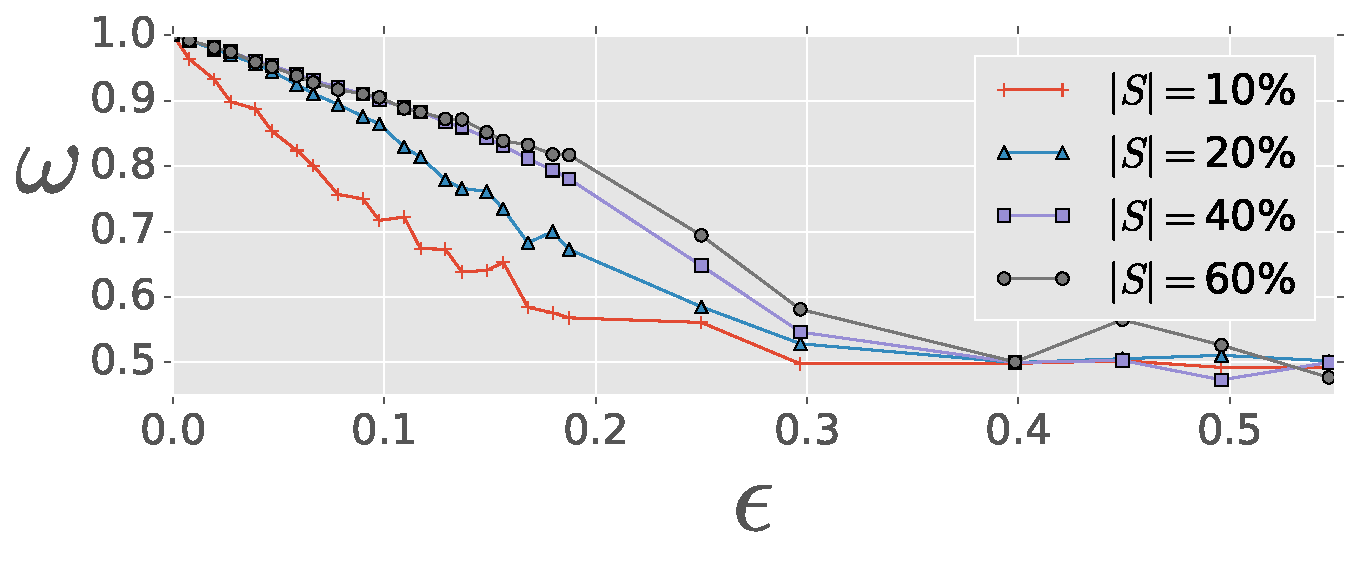
\includegraphics[scale=0.6]{figures/omega_vs_eps_dim8_nexp50_std_nEss8.pdf}
  \caption{$\omega$ for $\epsilon$-close functions to $L$.}
\label{omega_vs_eps}
\end{center}
\end{figure}

When $\epsilon = 0$ we get $\omega = 1$, as expected from
Proposition \ref{AP_is_L}. We observe an almost linear decrease in $\omega$ as
$\epsilon$ grows to $0.3$ then leading to a plateau where $\omega =
\frac{1}{2}$, indicating that the analogical labels $\albl{\mathbf{x}}_f$ are
more or less random. Moreover, $\omega$ appears to decrease faster for small
samples $S$. This is due to the fact that the analogical labels
$\albl{\mathbf{x}}_f$ are the result of a majority-vote procedure among the
candidate solutions that one can build from $S$, and the number of candidates
becomes smaller as $|S|$ decreases, thus altering the quality of the
prediction. The determination of a functional dependence between $\omega$,
$\epsilon$ and $|S|$ is currently being investigated.

Now, let us note the following point: even if a function $f$ is far from being
AP, the quality $\omega$ of the extension $\mathbf{E}_S(f)$ may still be very
high. To illustrate this, let us define the value $\beta$ which is an indicator
of how far is $f$ from being completely AP.  For each $\mathbf{x} \in
\mathbf{E}^*_S(f)$, we define $\beta_\mathbf{x}$ as the proportion of
candidates $y$ that led to the the correct label, i.e. the proportion of $y$
such that $y = f(\mathbf{x})$. $\beta$ is defined as the average of all the
$\beta_\mathbf{x}$.  Obviously, a function $f$ is AP iff $\beta = 1$ for all
$S$, i.e. if $\beta_\mathbf{x} = 1$ for all $\mathbf{x} \in \mathbf{E}^*_S(f)$
and for all $S$.

Table \ref{table_monks} reports the values of $\omega$ and $\beta$ for the
Standard and the Klein modelings of analogy (respectively $\omega_S$,
$\omega_K$, $\beta_S$ and $\beta_K$) over three datasets from the UCI
repository, namely the three Monk's problems\footnote{As these datasets are
nominally-valued, they are binarized.} \cite{UCIrepo}. Results are averaged
over 100 experiments, where the sample set $S$ is each time randomly sampled
with a size of $30$\% of the universe of possible instances.

\begin{table}
\centering
\begin{tabular}{| c | c | c | c | c |}
\toprule
  & $\omega_S$  & $\omega_K$ & $\beta_S$  &  $\beta_K$ \\
\midrule
Monk 1 & .96 & .96 & .73 & .62 \\
Monk 2 & .96 & .84 & .69 & .60 \\
Monk 3 & .98 & .95 & .87 & .77 \\
\bottomrule
\end{tabular}
\caption{$\omega$ and $\beta$ for the Standard and Klein modelings over the
  Monk's problems.}
\label{table_monks}
\end{table}

We observe that for each dataset, $\beta_S$ is significantly lower than $1$.
This suggests that the Boolean functions underlying these
datasets are highly not AP, because on average, there is a high proportion
(around $20$\%) of candidates $y$ that predicted the wrong label. However,
$\omega_S$ is no lower than $96$\%, implying extensions of very high quality.
This is where the majority-vote comes into play: in some cases, it may be able
to compensate for the predictors $y$ that were wrong.  This is what happens
here in $96$\%, $96$\% and $98$\% of the cases respectively. Here again,
obtaining theoretical guarantees about the majority vote procedure is currently
investigated.

We note also that the Klein modeling achieves equal or lower quality than the
standard one, which suggests that the Standard modeling, which has the same
class of AP functions, is more useful in practice. Note that such a difference
between $\omega_S$ and $\omega_K$ has been consistently observed over many
other experiments, which we do not mention here for lack of space. This may be
explained by the fact that, as mentioned earlier, the Klein modeling obeys
the following property, unnatural  for an analogy: $A_K(a, b, c, d)
\iff A_K(b, a, c, d)$.
